\section{Methodology}

\section{Workflow Overview}

The general methodology for this work is described in figure
\ref{fig:workflow}. Each portion of this figure is discussed in detail
in this section.

\begin{center}
  \begin{figure}
    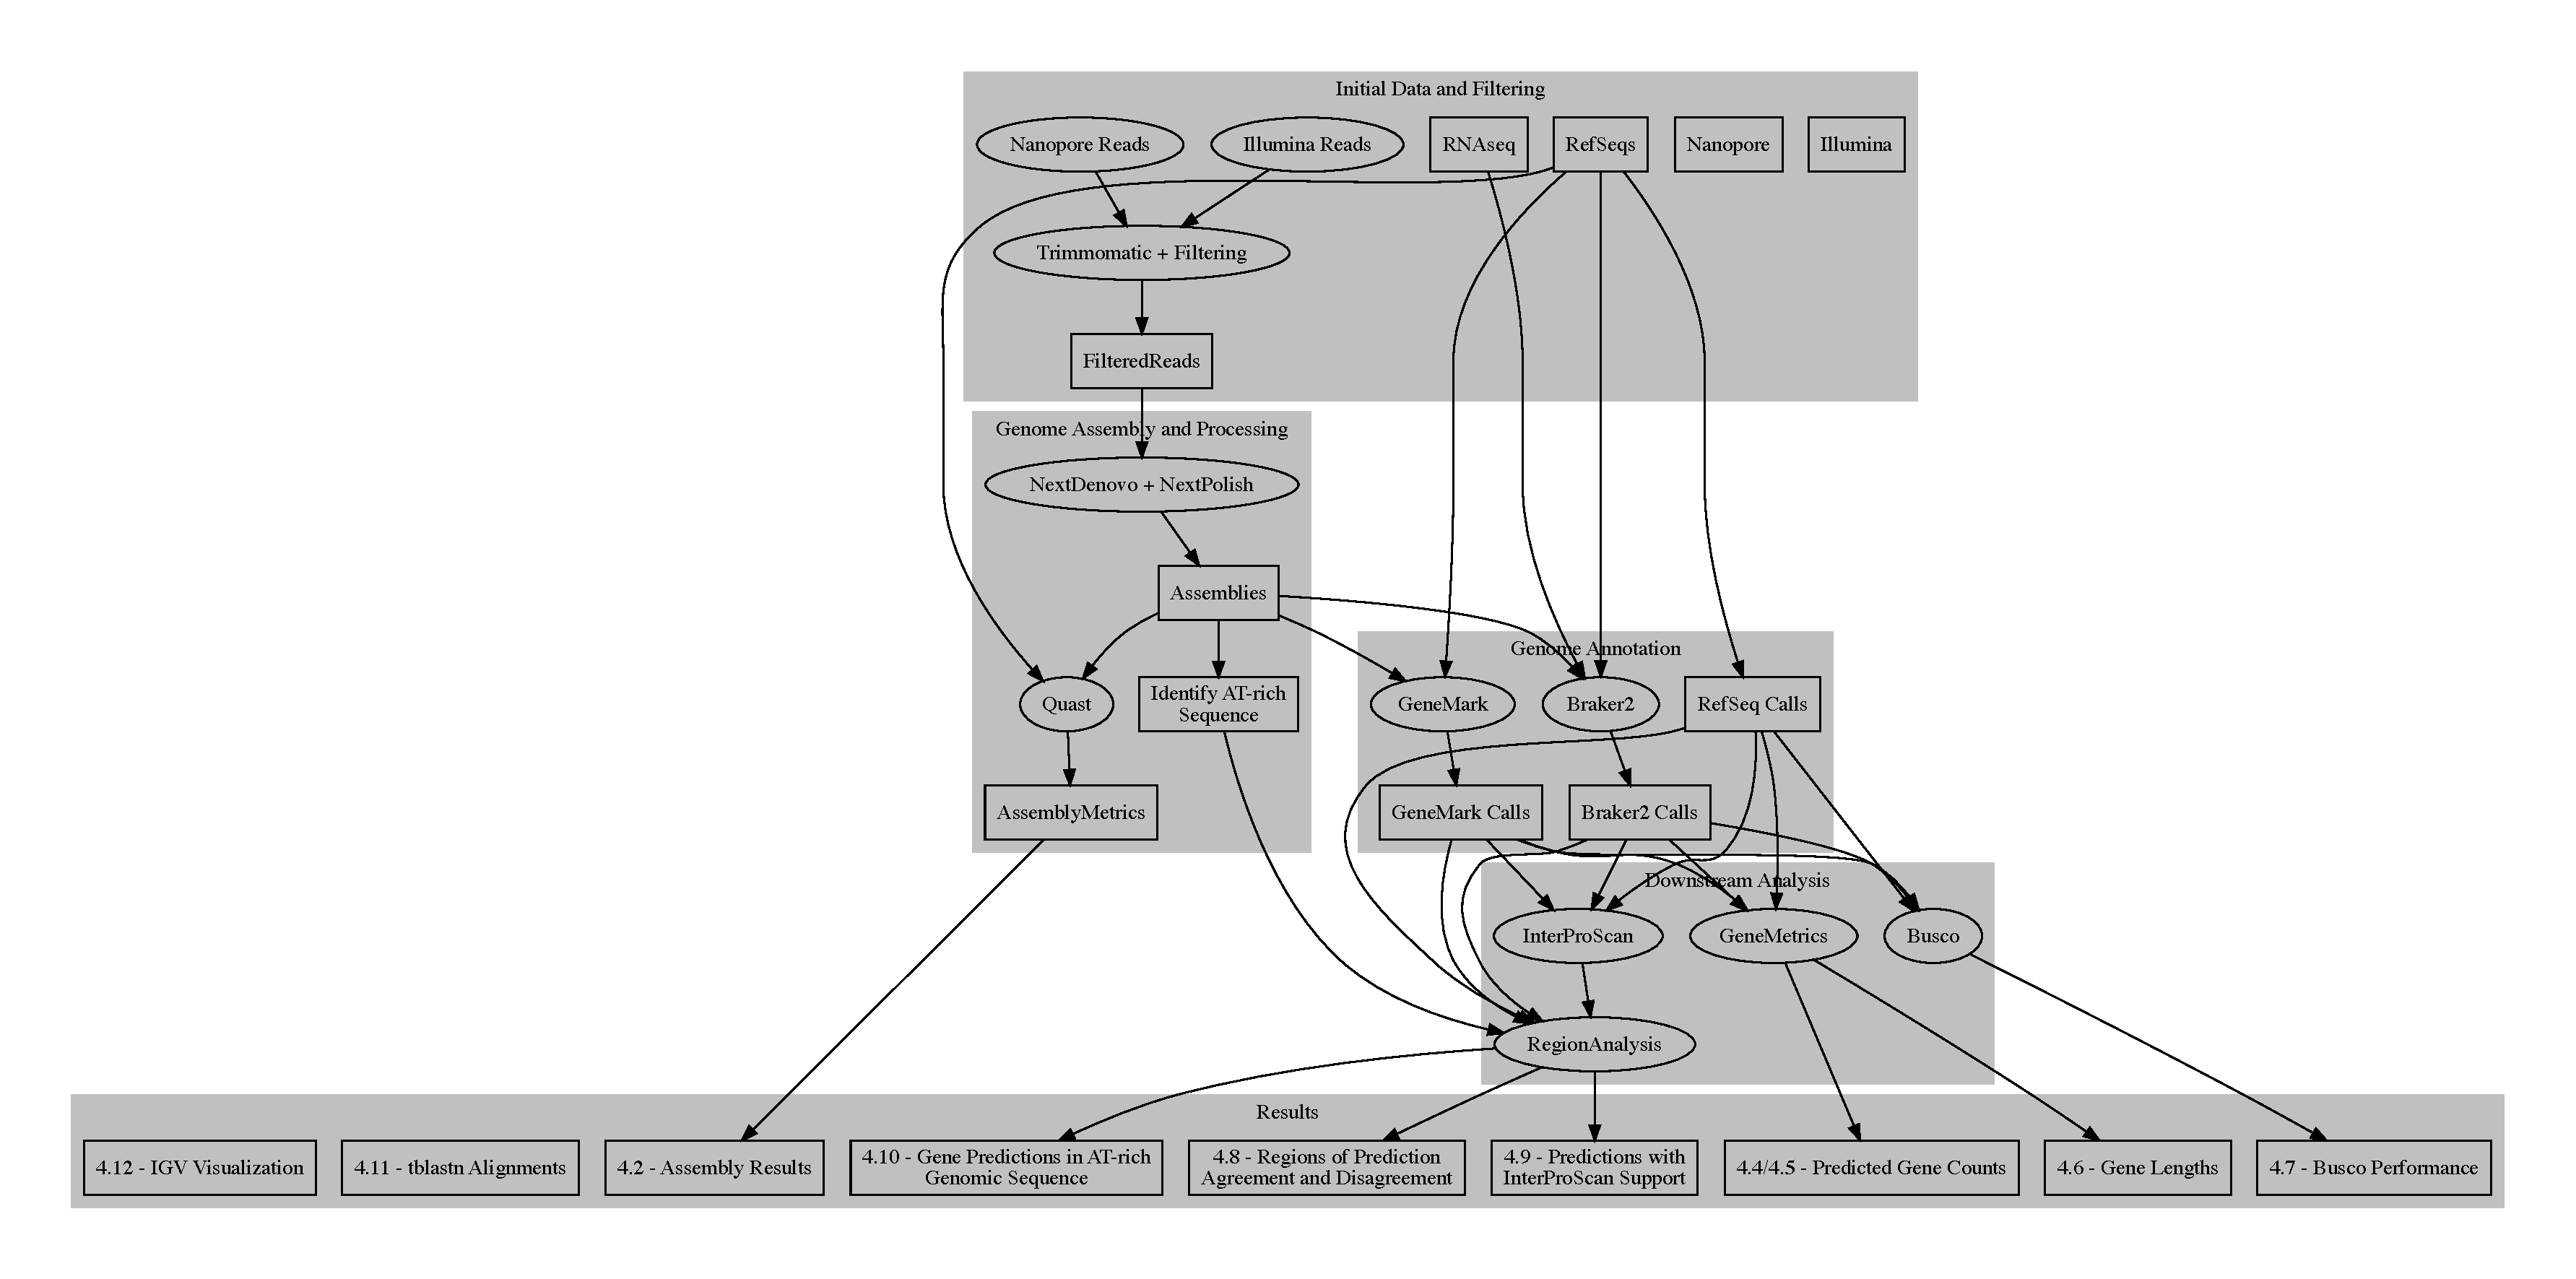
\includegraphics[width=1.15\textwidth]{./figures/data-flowchart.pdf}
    \caption{A flowchart of the methodology followed for this
      research. The workflow is broken up into sections based on the
      stage of the pipeline. Oval-shaped nodes represent steps
      involved in the processing of data, while rectangular nodes
      represent intermediate datasets and results.}
    \label{fig:workflow}
  \end{figure}
\end{center}
      
\section{Assembly and Annotation}

\subsection{Assembly}

Prior to gene prediction, genomic Nanopore sequences from DC1 and
Tsth20 were assembled in to contigs using NextDenovo\ref{Hu02024} and
then polished with Illumina sequences using
NextPolish\ref{Hu2020}. Assembly and polishing were both performed
using default parameters.

%In an attempt to produce high quality assemblies of DC1 and Tsth20, We
%decided on a set of tools named NextDenovo and NextPolish as they have
%produced excellent assemblies based on previous experience. (should
%find a citation to confirm this)

%(Might be better for discussion or omitted since it is specific to our
%setup) Initial attempts to run the example dataset resulted in
%permissions errors due to the management of the storage system being
%used, which were encountered with other tools in the past. To remedy
%this, the software installation was copied to RSMI's scratch space on
%Copernicus. Once the approriate permissions were given to run
%nextDenovo, the example dataset was run without issue.

%Following assembly using nextDenovo, Illumina sequence data from DC1
%and Tsth20 was used to polish each respective genome using
%nextPolish. Default parameters were used from assembly except for
%modification of the parallel option to reduce processing times.

%\subsection{Repeat Masking}

%In order to evaluate the performance of gene finding tools in
%repetitive or low complexity regions in the context of
%\textit{Trichoderma} genomes, we must first identify said regions in
%the genomes considered. To do this, the GenericRepeatFinder tool was
%used, which is a \textit{de novo} repeat detection tool
%\cite{10.1104/pp.19.00386}. GenerifRepeatFinder detects three
%different types of repeats, those being MITEs, TDRs and TIRs. Commands
%used for this program follow the example commands provided on the
%GitHub page for the GenericRepeatFinder project.

\subsection{Gene prediction with GeneMark-ES}

GeneMark-ES was run as it requires no prior information or alignments
in order to run. In this case GeneMark-ES has an option specifically
for fungal genomes, which was used in this case. Apart from the fungal
option, the only additional options supplied were for output format of
GFF3 and number of cores for reduced processing time.

General command structure for GeneMark-ES:

gmes\_petap.pl --ES --fungus
--format gff3 --cores 48 --sequence /path/to/sequence

\subsection{Braker2}

As mentioned previously, \textit{Trichoderma reesei} was selected as
the \'reference\' genome for this work. With this in mind, several
short read archives (SRAs) from \textit{T. reesei} were selected for
Augustus training. Following Augustus training, the model for
\textit{T reesei} was applied to all genomes considered. Settings and
procedures from running Braker2 are described below.

The variables that need to be set are AUGUSTUS\_CONFIG\_PATH and
TSEBRA\_PATH. Augustus, by defuault, tries to write species
information to the location where the software is installed. In this
case, we don'thave write permissions to the compute canada software
stack hosted byt Research Computing, so the AUGUSTUS\_CONFIG\_PATH
variable must be set in order to create a writeable directory. As long
as that path has a directory within it called braker, and a species
directory within the braker directory, things should go
smoothly. TSEBRA is a set of scripts also made by the creators of
Braker and is required to merge results from the various gene
prediction tools involved in the Braker2 pipeline. The TSEBRA\_PATH
simply points to the directory where TSEBRA is located Both Braker2
and TSEBRA can be cloned directly from GitHub (links to come)

\section{Identification of Overlapping Features and Regions}

Feature Identification: To first undertand how gene prediction tools
perform in comparison to other gene prediction tools, we must identify
features. This identification of features will help us descirbe the
similarities, and differences between gene finding tools. A feature,
in this context, is any feature stated within a Genomic Feature Format
file (GFF) provided to the program, in which mutliple GFF files can be
provided. The definition of a feature, for this application, is an
object that contains a contig ID, a start position, an end position
and a strand property. In the context of features on different
strands, start and stop positions of features are sorted based on left
and right positions of the feature in respect to the reference
sequence.

Region Identification: In addition to feature creation, we will also
identify regions of overlapping features based on the precitions from
each gene finding tool. These regions will help identify the
agreements, or disagreements, between different gene-finding tools. A
region, in this context, is a set of overlapping features, all of
which overlap at least one other feature in the region. With each
overlap, there will be an overlap type. These types can be defined
based on Allen's Interval Calculus (reference), with the exception of
features that start beyond the end point of the current region.

=======
Example command for braker2:

/scratch/p2irc/p2irc\_rsmi/cbe453/masters/software/braker2/BRAKER/scripts/braker.pl
--gff3 --threads 60
--TSEBRA\_PATH=/scratch/p2irc/p2irc\_rsmi/cbe453/masters/software/braker2/tsebra/TSEBRA/bin/
--genome /path/to/sequence --species=TreeseiFungal --fungus
--useexisting

BUSCO methodology (from research questions)
The BUSCO method was applied using two BUSCO subsets,
one generally applicable for fungi, and another targeting an
evolutionary branch more closely related to \textit{Trichoderma}.

Stats for length analysis (from research questions)
The first statistical tool to be applied is ANOVA (analysis of
variance) to compare the mean lengths genes predicted by each gene
finding tool with the null hypothesis being that the mean of predicted
gene lengths should be the same across all tools considered. In
addition to ANOVA, pairwise comparisons of the distributions using a
Kolmogorov–Smirnov test is appropriate. The null hypothesis in this
test would be that the gene lengths are sample from the same
distribution.

Stats for binomial tests (from research questions)
To do this, a binomial test will be used, with the null hypothesis
being that the number of genes predicted in regions of normal and
abnormal GC content should be proportional to the length of normal and
abnormal GC content regions in the assembly. For example, if 30
percent of the genome is comprised of anomalous GC content, then we
would expect 30 percent of predicted genes to be present in those
regions. In addition to anomalous GC content, this test can be applied
to repetitive content in assemblies as well.

Stats for regions (from research questions)
From these results, Venn diagrams will be generated with
Jaccard index calculated for each combination of gene finding
tools. The region identification process can also be extended to
include features identified by other tools, such as BLAST hits to
validated gene models from other organisms and small RNAs. Chi2
goodness of fit tests can then be applied to counts of 'validated'
gene predictions or other features with the same null hypothesis that
gene finders should predict the same number of features.
